% \subsection{Propagation}
Propagation is one of the fundamental pillars of constraint programming, along with modeling and search.
Global constraints spanning a large number of variables allows one to leverage propagation to the fullest.
The application of propagation to the problem of OCL is our fundamental difference to much of the related work.
To apply it to OCL we need a systematic way to model OCL expressions using gobal constraints, and particularly to model OCL query expressions.


\subsection{Local Consistency}
\ytodo{Local Consistency is around a single constraint, enforced/checked by its propagation algorithm}

\begin{figure}[!ht]
    \centering
    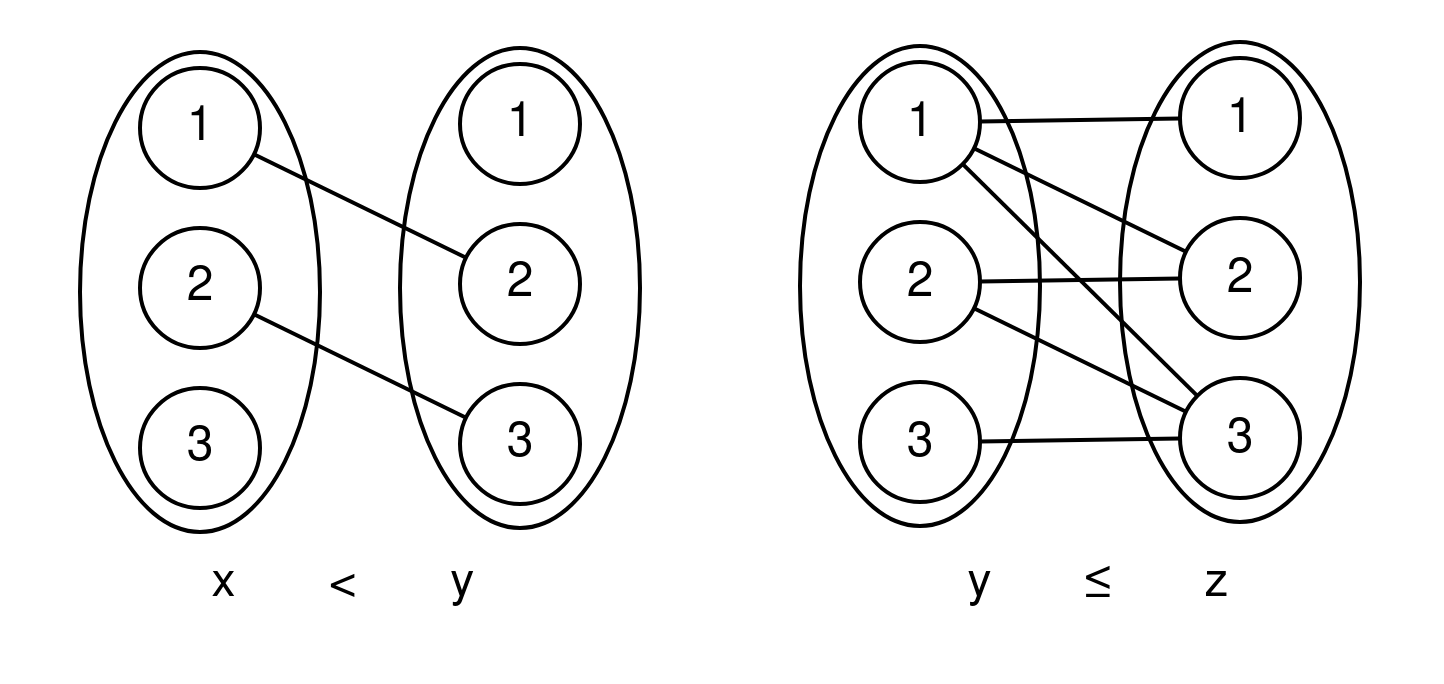
\includegraphics[trim={0 0 0 0},width=0.5\linewidth]{Context/CP/figures/local.png}
    \caption{Illustration of Generalized Arc Consistency and Bound Consistency on $x<y\leq z$}
    \label{fig:GACandBC}
\end{figure}
In this figure we see local consistency enforced over the expressions $X<Y$ and $Y\leq Z$.
For every possible value of each domain, we can find at least one value in the other domain(s) which satisfy the constraint.

\subsection{Generalized Arc Consistency and Bound Consistency}
\ytodo{General Arc Consistency is ideal, Bound Consistency is reasonable}
\ytodo{These generalized consistencies can be approched by combining local consistencies}
\begin{figure}[!ht]
    \centering
    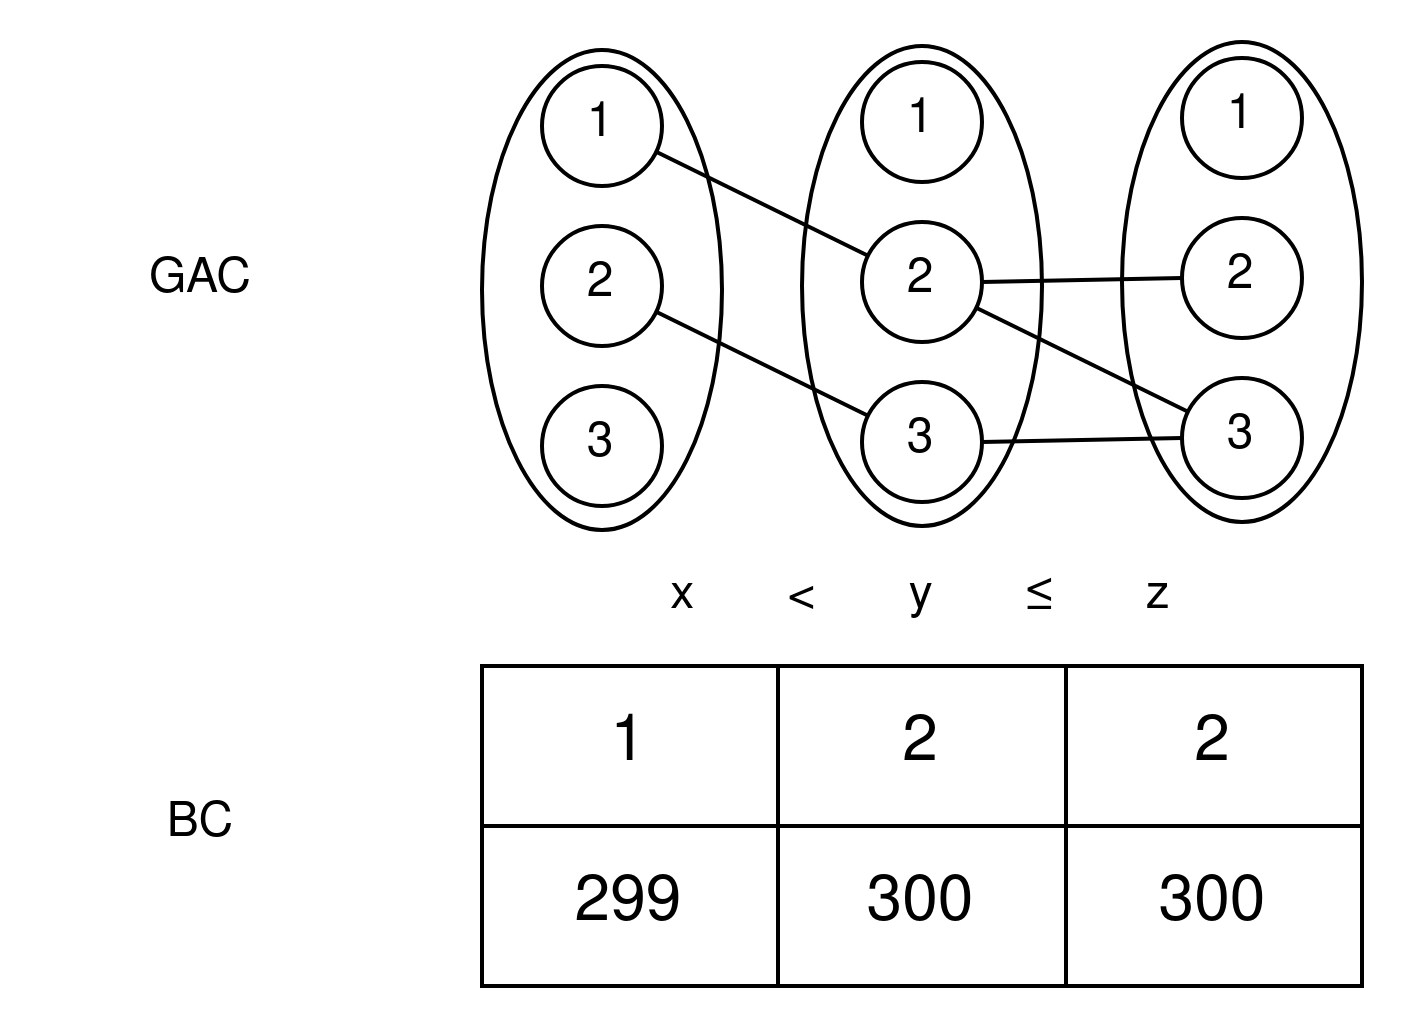
\includegraphics[trim={0 0 0 0},width=0.5\linewidth]{Context/CP/figures/GACandBC.png}
    \caption{Illustration of Generalized Arc Consistency and Bound Consistency on $x<y\leq z$}
    \label{fig:GACandBC}
\end{figure}
In this figure we illustrate \textit{generalized arc consistency} (GAC) above and \textit{bound consistency} (BC) below, for the CSP: $x<y\leq z$.
To illustrate the advantage of bound consistency we extended the domain from [1..3] to [1..300], making it 100 times bigger while keeping the same encoding.
For generalized arc consistency, we can see the enumerated domains of $X$, $Y$ and $Z$.
Across the domains of the variables, we link possible valuations satisfying the whole problem: for instance if $X=1$, we are connected to two valid assignments for $Y$ and $Z$.
Bound consistency on the other hand, only requires an encoding of the upper and lower bounds of the domain, for which it maintains consistency in the same way as GAC.



% \subsection{Propagation on boolean variables and CNF models}
% \ytodo{DDPL is a propagator for the gobal constraint "CNF model"}

% \subsection{Propagation on real variables and systems of linear equations}
% \ytodo{Simplex is a propagator for the gobal constraint "system of linear equations"}